% !Mode:: "TeX:UTF-8"
%!TEX program  = xelatex

\documentclass[withoutpreface,bwprint]{cumcmthesis}

\usepackage{mathrsfs}

\coursename{ACM-ICPC 算法与程序设计}
\title{基于不相交集的问题求解报告}
\schoolname{微电子与固体电子学院}
\studentid{2016030102010}
\xuankehao{}
\author{傅宣登}
\theteacher{杨鹏}

\begin{document}
\maketitle
\begin{abstract}

不相交集是一种常用的数据结构。这种数据结构实现简单,操作迅速。

简单地说,不相交集可用于快速查询一堆元素是否属于同一集合。
鉴于在有些问题中,这种关系相当隐秘,本文采用另一种更理论的方式来描述这种关系。

本文讨论了实现不相交集的基础数据结构:数组、红黑树、树。本文采用树来实现不相交集。
接着给出了朴素的求并、查询算法,然后用所谓的路径压缩优化了查询算法。

最后为说明并查集在具体问题中的应用,给出了一道例题,并提供了完整的求解报告。

在附录中给出了校赛的账号和密码。

\keywords{不相交集\quad  算法\quad   数据结构\quad  程序设计}
\end{abstract}

\begin{center}%
	{\zihao{4}\heiti 正文 \vspace{-.5em}}%
\end{center}%

\section{不相交集 ADT}

不相交集(并查集)是描述解决等价问题的一种有效数据结构。
这种数据结构实现起来非常简单,而且每种操作只需要常数平均时间。
许多算法中都用到了不相交集,例如 \verb|Kruskal| 算法和 \verb|Prim| 算法等。

\subsection{等价关系}

若对每一对元素 $(a, b),\ \ a,b \in S$,$aRb$ 要么为 \verb|true| 要么为 \verb|false|,
则称在集合 $S$ 上定义关系 $R$。
如果 $aRb$ 是 \verb|true|,那么我们说 $a$ 与 $b$ 有关系。

\begin{definition}[等价关系]
等价关系是满足下列三个性质的关系 $R$:
\begin{itemize}
\item (自反性)对于所有的 $a\in S$,$aRa$;
\item (对称性)$aRb$ 当且仅当 $bRa$;
\item (传递性)若 $aRb$ 且 $bRc$,则 $aRc$。
\end{itemize}
\end{definition}

这里有几个例子。

如果两个城市位于同一个国家,那么定义他们是有关系的。容易验证这是一个等价关系。
如果能够通过公路从城镇 $a$ 旅行到 $b$,则设 $a$ 与 $b$ 有关系。
如果所有的道路都是双向行驶的,那么这种关系也是一个等价关系。

\subsection{动态等价性问题}

给定一个等价关系“$\sim$”,一个自然的问题是对任意的 $a$ 和 $b$,确定是否 $a\sim{}b$。
如果将等价关系存储为一个二维布尔数组,那么当然这个工作可以以常数时间完成。
问题在于这种关系的定义通常不明显甚至相当隐秘。

例如,设在5个元素的集合 $\{a_1,a_2,a_3,a_4,a_5\}$ 上定义一个等价关系。
此时存在25对元素,他们的每一对要么有关系要么没有关系。
然而,信息 $a_1\sim{}a_2, a_3\sim{}a_4, a_4\sim{}a_2, a_1\sim{}a_5$ 意味着每一对元素都是有关系的。
我们需要一个能快速判断出这些关系的数据结构。

\begin{definition}[等价类]
一个元素 $a\in{}S$ 的等价类是 $s$ 的一个子集,它包含所有与 $a$ 有关系的元素。
\end{definition}

显然,等价类形成对 $S$ 的一个划分:$S$ 的每一个元素恰好出现在一个等价类中。
这样,为确认是否 $a\sim{}b$,我们只需验证 $a$ 和 $b$ 是否都在同一个等价类中。

输入数据最初是由 $N$ 个集合的类,每个集合含有一个元素。
初始的描述是所有的关系均为假(自反的关系除外)。
每个集合都有一个不同的元素,从而 $S_i\cap{}S_j = \varPhi$;
即所有集合不相交。

此时,我们定义两种运算。
第一种是 \verb|Find|,它返回包含给定元素的集合(即等价类)的名字。
第二种是添加关系。
如果我们想要添加关系 $a\sim{}b$,那么我们首先要看是否 $a$ 和 $b$ 已经有关系。
这可以通过对 $a$ 和 $b$ 执行 \verb|Find| 并检查它们是否在同一个等价类中来完成。
如果它们不在同一个等价类中,那么我们使用求并运算 \verb|Union|,这种运算把含有 $a$ 和 $b$ 的两个等价类合并成一个新的等价类。
从集合的观点看,$\cup$ 的结果是建立一个新集合 $S_k = S_i \cup S_j$,并去掉原来两个集合而保持所有的集合的不相交性。
由于这个原因,常常把这项工作的算法叫做不相交集的 \verb|Union|/\verb|Find| 算法,不相交集也叫并查集。

很容易观察到,该算法是动态的。因为在算法执行的过程中,集合可以通过 \verb|Union| 运算而发生变化。
另外,由 \verb|Find| 返回的集合的名字实际上是相当任意的。
真正重要的关键在于:当 $a$ 和 $b$ 在同一个集合中的时候,$\mathrm{Find}(a) = \mathrm{Find}(b)$。

解决动态等价性问题的方案有两种。
一种方案保证指令 \verb|Find| 能够以常数最坏情形运行时间执行,
而另一种方案则保证指令 \verb|Union| 能够以常数最坏情形运行时间执行。
曾有人指出二者不能同时做到。

\section{不相交集的实现}

本文将考查 \verb|Union|/\verb|Find| 问题的一种解法,
其中每次操作的执行时间几乎是常数时间。

\subsection{基本数据结构}

%\subsubsection{容器的选择}
注意到动态等价性问题并不要求 \verb|Find| 操作返回任何特定的名字,
而只是要求当且仅当两个元素属于同一个集合时,
作用在这两个元素上的 \verb|Find| 返回相同的名字。

于是有多种容器可以用来实现并查算法,例如树、数组(向量)、集合(红黑树)等,
本文仅讨论使用树来表示集合的实现方法。
由于树上每一个元素都有相同的根,
这样该根就可以用来命名所在的集合。

虽然这些树不一定是二叉树,但要表示他们却相当的容易,因为需要存储的唯一信息就是一个父指针。
集合的名字由根节点给出。
可以用一个数组存储这些树,数组中每个成员 $P[i]$ 表示元素 $i$ 的父节点。
如果 $i$ 是根,那么 $P[i] = i$。

初始时,对于 $1\le i \le N,\,{}P[i] = i$。

\subsection{并查算法}

对元素 $X$ 执行 $\mathrm{Find}(X)$ 操作会返回包含 $X$ 的的树的根,
这可以通过不断对它的父节点执行 \verb|Find| 操作完成。
\begin{lstlisting}{language=C}
Find(x):
	if P[x] == x
		return x;
	else
		return Find(P[x]);
\end{lstlisting}
执行这次操作的时间与表示 $X$ 的节点的深度成正比。

为了执行两个元素的 \verb|Union| 运算,只需使一个节点的根指向另一棵树的根节点。
\begin{lstlisting}{language=C}
Union(x, y):
	P[ Find(x) ] = P[ Find(y) ];
\end{lstlisting}

上面伪代码表示的基本算法的实现中,假设差错检验已经执行。

\subsection{路径压缩}

如果存在大量对深节点的 \verb|Find| 操作,
那么将重复执行很多次相同的递归调用,这是非常浪费时间的。
于是可以考虑每次执行 \verb|Find| 操作时,
将该节点的根节点修改为其树的根节点,以减少将来访问的时间。

\begin{lstlisting}{language=C}
Find(x):
	if P[x] == x
		return x;
	else
		return P[x] = Find(P[x]);
\end{lstlisting}

优化后的算法在最坏情形下几乎是线性的。在最坏情况下需要的时间是
$\Theta(M\alpha(M,N))$ (假设 $M\ge N$),
其中 $\alpha(M, N)$ 是 Ackermann 函数的逆。

\section{例题:TROY Query}

本文以 Codeforces Hello 2015 (Div. 2) 的 F 题\footnote{http://codeforces.com/gym/100571/problem/F}为例,
展示并查集在实际问题中的综合与应用。

\subsection{问题大意}

给出一个 $10^{18} \times 10^{18}$ 的棋盘,
每个格子里要么是 $+1$、要么是 $-1$。
对这个棋盘可以执行两种操作:

\begin{enumerate}
\item 将一行中的所有格子里的数乘以 $-1$ .
\item 将一列中的所有格子里的数乘以 $-1$ .
\end{enumerate}

现在有两个这样的棋盘,记为 $a$ 和 $b$。
初始时两个棋盘上的所有格子都未知。
现在有若干次询问,每次询问告诉你两个棋盘上第 $x$ 行、第 $y$ 列的格子分别是什么。
你需要指出在当前已知的信息下,能否通过若干次操作使 $a$ 变成 $b$。
需要注意的是每次询问已知的信息是累计的,
对于未知的格子应当假设它们的值是使变换可能(如果可能)的值。

询问最多 $10^5$ 个,且有 $1\le x,y \le 10^{18}$。

\subsection{问题分析}

首先我们注意到,对每行或每列的执行操作的次数和顺序是不重要的,
唯一需要关注的是执行操作的次数的奇偶,也就是该行(列)的元素最终有没有被反号。

现在用 $R(x)$ 表示第 $x$ 行最终没有被反号,用 $C(y)$ 表示第 $y$ 列最终没有被反号。
同时 $\neg R(x)$ 和 $\neg C(y)$ 表示第 $x$ 行或第 $y$ 列最终反号了。

然后考虑某一个格子 $(x,y)$。

如果 $a_{x,y} = b_{x,y}$,那么变换后 $a$ 中对应的格子必须不变,
也即是 $R(x)$ 和 $C(y)$ 必须同时成立,或者 $\neg R(x)$ 和 $\neg C(y)$ 同时成立。
我们用 $\sim$ 表示同时成立,上述限制也即是 $R(x) \sim C(y)$ 或 $\neg{}R(x)\sim\neg{}C(y)$。
这其实是一种等价关系。

同理,如果 $a_{x,y} \ne b_{x,y}$,
那么 $R(x) \sim\neg C(y)$ 或 $\neg{}R(x)\sim{}C(y)$。

显然,如果在某次查询后,
存在一个 $x$ 使得 $R(x)\sim\neg{}R(x)$ 或 $C(x)\sim\neg{}C(x)$,
那么从 $a$ 到 $b$ 的变换就不可能了,并且对于以后的所有查询也是不可能。

很显然,这是一类动态等价性的问题,可以用并查集来解决。

但此时还有一个问题,$x,y$ 高达 $10^{18}$,
用数组表示并查集的话,则需要 $4\times{}10^{18}$ 个元素。
256兆的内存是开不下这么大的数组的。
注意到询问最多只有 $10^5$ 个,这样不相同的 $x$ 或 $y$ 最多 $10^5$ 个。
因此可以做一次离散化使 $x$ 和 $y$ 变小,这样就最多只用开一个 $4\times{}10^5$ 的数组了。

\subsection{解决方案}

顺序读取每个查询,把大坐标映射成一个小的虚拟坐标,
只要相同的行或列映射成相同的虚拟行(列)坐标即可。

\newcommand\mX{\mathscr{X}}
\newcommand\mY{\mathscr{Y}}
\newcommand\mU{\mathrm{Union}}
\newcommand\mF{\mathrm{Find}}

对于虚拟坐标 $(\mX,\:\mY)$,
分别用数字
$2\mX-1$、$2\mX$、$\mathcal{MAXT}-2\mY$、$\mathcal{MAXT}-2\mY+1$
表示
$R(\mX)$、$\neg{}R(\mX)$、$C(\mY)$、$\neg{}C(\mY)$。

如果 $a_{\mX,\mY} == b_{\mX,\mY}$,
则执行 $\mU(R(\mX),\:{}C(\mY))$ 和 $\mU(\neg{}R(\mX),\:\neg{}C(\mY))$。
如果 $a_{\mX,\mY} \ne b_{\mX,\mY}$,
则执行 $\mU(R(\mX),\:\neg{}C(\mY))$ 和 $\mU(\neg{}R(\mX),\:{}C(\mY))$。

之后检查是否有 $R(\mX)\sim\neg{}R(\mX)$ 或 $C(\mY)\sim\neg{}C(\mY)$。
若有则变换不可能,且之后所有询问都不可能。
否则当前询问后变换可能,继续处理下一个询问。

\subsection{实现与评测}

使用 C++ 实现上述解法\footnote{具体代码请见\ref{cppsource}},
提交并通过了 Codeforces 的测评,如图\ref{verdicp}。

\begin{figure}[!h]
\centering
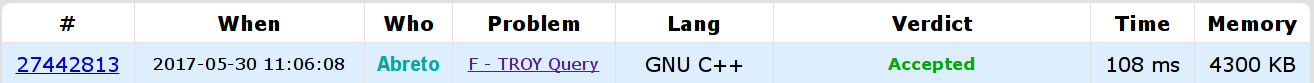
\includegraphics[width=\textwidth]{v.png}
\caption{测评结果}\label{verdicp}
\end{figure}

%参考文献
\bibliographystyle{unsrt}
\nocite{*}
\bibliography{reference}

\newpage
%附录
\appendix
\section{TROY Query 源代码}\label{cppsource}
\lstinputlisting[language=C++]{src/troy.cpp}

\section{OJ 帐号与密码}

OJ 帐号实在太多,故仅列出部分。以下密码在 2017 年 07 月 01 日前有效。

%SpecialPWD,by0701.
\begin{table}[h]
\centering
\begin{tabular}{cccc}
 \hline
 \makebox[0.1\textwidth][c]{OJ}	& \makebox[0.3\textwidth][c]{链接} & \makebox[0.1\textwidth]{帐号} & \makebox[0.2\textwidth]{密码} \\ \hline
 cdoj & http://mozhu.today & \verb|abreto| & \verb|SpecialPWD,by0701.| \\ \hline
 codeforces & http://abreto.cf & \verb|Abreto| & \verb|SpecialPWD,by0701.| \\ \hline
 AtCoder & http://atcoder.jp & \verb|abreto| & \verb|SpecialPWD,by0701.| \\ \hline
 Virtual Judge & https://vjudge.net & \verb|Abreto| & \verb|SpecialPWD,by0701.| \\ \hline
\end{tabular}
\caption{部分 OJ 帐号与密码}
\end{table}

特别的,校赛帐号是 \verb|15th_team067|,密码是 \verb|aIbv8f0J|,决赛排名42,获二等奖。

\end{document}
